\section{Transportlagstjenester og protokoller (3.1)}
%=============================================================================

\subsection{Transportlagets rolle}

\begin{keybox}[Transportlaget -- oversikt]
Transportlaget tilbyr \textbf{logisk kommunikasjon} mellom \emph{applikasjonsprosesser} p\aa\ forskjellige verter (hosts).
\begin{itemize}[noitemsep]
    \item Sendersiden: bryter applikasjonsmeldinger i \textbf{segmenter}, sender dem til nettverkslaget
    \item Mottakersiden: setter segmenter sammen til meldinger, leverer til applikasjonslaget
    \item To hovedprotokoller: \textbf{TCP} og \textbf{UDP}
\end{itemize}
\end{keybox}

\subsection{Transportlag vs. nettverkslag}

\begin{keybox}[Viktig forskjell]
\begin{itemize}[noitemsep]
    \item \textbf{Nettverkslag (IP):} Logisk kommunikasjon mellom \emph{verter} (hosts)
    \item \textbf{Transportlag (TCP/UDP):} Logisk kommunikasjon mellom \emph{prosesser}
    \item Transportlaget utvider nettverkslagets host-til-host-levering til prosess-til-prosess-levering
\end{itemize}
\end{keybox}

\begin{warnbox}[Husholdningsanalogi]
Tenk p\aa\ to hus med 12 barn i hvert hus som sender brev til hverandre:
\begin{itemize}[noitemsep]
    \item \textbf{Prosesser} = barn
    \item \textbf{Applikasjonsmeldinger} = brev i konvolutter
    \item \textbf{Verter (hosts)} = hus
    \item \textbf{Transportprotokoll} = Ann og Bill (barna som samler/sorterer post)
    \item \textbf{Nettverkslagsprotokoll} = postvesenet
\end{itemize}
Ann og Bill jobber innenfor huset -- de kan ikke kontrollere hva som skjer ute i postsystemet.
\end{warnbox}

\subsection{Internettets transportprotokoller}

\begin{keybox}[TCP vs. UDP -- oversikt]
\textbf{TCP (Transmission Control Protocol):}
\begin{itemize}[noitemsep]
    \item P\aa litelig, ordnet levering (\emph{reliable, in-order delivery})
    \item Metningskontroll (\emph{congestion control})
    \item Flytkontroll (\emph{flow control})
    \item Tilkoblingssoppsett (\emph{connection setup})
\end{itemize}

\textbf{UDP (User Datagram Protocol):}
\begin{itemize}[noitemsep]
    \item Up\aa litelig, uordnet levering (\emph{unreliable, unordered delivery})
    \item Ingen metningskontroll, flytkontroll eller tilkoblingsoppsett
    \item ``Best effort'' -- ingen garanti p\aa\ levering
\end{itemize}

\textbf{Tjenester som IKKE tilbys:} Forsinkelses- eller b\aa ndbreddegarantier.
\end{keybox}

%=============================================================================
\section{Multipleksing og demultipleksing (3.2)}
%=============================================================================

\subsection{Grunnleggende konsept}

\begin{keybox}[Multipleksing og demultipleksing]
\textbf{Multipleksing hos sender:}
\begin{itemize}[noitemsep]
    \item H\aa ndterer data fra flere sokler (sockets)
    \item Legger til transportheader (med portnummer) for \aa\ identifisere sokkel
\end{itemize}

\textbf{Demultipleksing hos mottaker:}
\begin{itemize}[noitemsep]
    \item Bruker headerinformasjon (portnummer) for \aa\ levere segmenter til riktig sokkel
\end{itemize}
\end{keybox}

\subsection{Hvordan demultipleksing fungerer}

\begin{itemize}[noitemsep]
    \item Verten mottar IP-datagrammer -- hvert datagram har kilde-IP, destinasjons-IP og ett transportlags-segment
    \item Hvert segment har \textbf{kilde-portnummer} og \textbf{destinasjons-portnummer} (16 bit hver)
    \item Verten bruker IP-adresser og portnumre for \aa\ dirigere segmentet til riktig sokkel
\end{itemize}

\begin{center}
\begin{tikzpicture}[scale=0.8]
    \draw[fill=lightblue] (0,0) rectangle (8,1.5);
    \draw (2,0) -- (2,1.5);
    \draw (4,0) -- (4,1.5);
    \node at (1,0.75) {\small Kilde-port};
    \node at (3,0.75) {\small Dest.-port};
    \node at (6,0.75) {\small Andre header-felt};
    \draw[fill=lightgreen] (0,-1.5) rectangle (8,0);
    \node at (4,-0.75) {\small Applikasjonsdata (payload)};
    \draw[decorate,decoration={brace,amplitude=5pt,mirror}] (0,-1.7) -- (2,-1.7) node[midway,below=5pt]{\tiny 16 bit};
    \draw[decorate,decoration={brace,amplitude=5pt,mirror}] (2,-1.7) -- (4,-1.7) node[midway,below=5pt]{\tiny 16 bit};
\end{tikzpicture}
\end{center}

\subsection{Tilkoblingsl\o s demultipleksing (UDP)}

\begin{keybox}[UDP-sokkel identifiseres av 2-tuppel]
UDP-sokkel identifiseres av: \textbf{(destinasjons-IP, destinasjons-port)}
\begin{itemize}[noitemsep]
    \item Segmenter med \emph{samme} destinasjons-IP og destinasjons-port, men \emph{forskjellig} kilde-IP/port, dirigeres til \textbf{samme sokkel}
    \item Kilde-port brukes som ``returadresse''
\end{itemize}
\end{keybox}

\subsection{Tilkoblingsorientert demultipleksing (TCP)}

\begin{keybox}[TCP-sokkel identifiseres av 4-tuppel]
TCP-sokkel identifiseres av: \textbf{(kilde-IP, kilde-port, destinasjons-IP, destinasjons-port)}
\begin{itemize}[noitemsep]
    \item Mottaker bruker \emph{alle fire verdier} for \aa\ dirigere segmentet til riktig sokkel
    \item Serververten kan st\o tte mange samtidige TCP-sokler -- hver identifisert med sin egen 4-tuppel
    \item Webservere har ulike sokler for hver klient (ulik kilde-IP og/eller kilde-port)
\end{itemize}
\end{keybox}

\begin{warnbox}[Viktig forskjell UDP vs. TCP demux]
\begin{itemize}[noitemsep]
    \item \textbf{UDP:} Kun destinasjons-port avgj\o r hvilken sokkel som f\aa r segmentet
    \item \textbf{TCP:} B\aa de kilde og destinasjon (IP + port) avgj\o r sokkel -- to klienter med ulik kilde-IP/port f\aa r \emph{separate} sokler
\end{itemize}
\end{warnbox}

%=============================================================================
\section{Tilkoblingsl\o s transport: UDP (3.3)}
%=============================================================================

\subsection{UDP -- oversikt}

\begin{keybox}[UDP -- User Datagram Protocol (RFC 768)]
\begin{itemize}[noitemsep]
    \item ``Bare bein'' transportprotokoll -- ``no frills''
    \item \textbf{Best effort}: Segmenter kan g\aa\ tapt eller leveres i feil rekkef\o lge
    \item \textbf{Tilkoblingsl\o s:} Ingen h\aa ndtrykk mellom sender og mottaker, hvert segment h\aa ndteres uavhengig
\end{itemize}

\textbf{Hvorfor brukes UDP?}
\begin{itemize}[noitemsep]
    \item Ingen tilkoblingsoppsett (som gir forsinkelse)
    \item Enkel: ingen tilstand i sender/mottaker
    \item Liten header (8 byte vs. 20 byte for TCP)
    \item Ingen metningskontroll -- kan sende s\aa\ raskt som \o nsket / applikasjonen tillater
\end{itemize}
\end{keybox}

\subsection{Bruksomr\aa der for UDP}

\begin{itemize}[noitemsep]
    \item Streaming av multimedia (tolererer tap, hastighetssensitiv)
    \item DNS (raske, korte foresp\o rsler)
    \item SNMP (nettverksadministrasjon)
    \item HTTP/3 (bruker QUIC over UDP)
\end{itemize}

\begin{warnbox}[UDP og p\aa litelighet]
Hvis p\aa litelig overf\o ring er n\o dvendig over UDP, m\aa\ det legges til i \textbf{applikasjonslaget}. Eksempel: HTTP/3 / QUIC legger til p\aa litelighet og metningskontroll over UDP.
\end{warnbox}

\subsection{UDP-segmentformat}

\begin{center}
\begin{tikzpicture}[scale=0.85]
    \draw[fill=lightblue] (0,2) rectangle (3,3);
    \draw[fill=lightblue] (3,2) rectangle (6,3);
    \node at (1.5,2.5) {\small Kilde-port \#};
    \node at (4.5,2.5) {\small Dest.-port \#};

    \draw[fill=lightblue] (0,1) rectangle (3,2);
    \draw[fill=lightblue] (3,1) rectangle (6,2);
    \node at (1.5,1.5) {\small Lengde};
    \node at (4.5,1.5) {\small Sjekksum};

    \draw[fill=lightgreen] (0,-0.5) rectangle (6,1);
    \node at (3,0.25) {\small Applikasjonsdata (payload)};

    \draw[decorate,decoration={brace,amplitude=5pt}] (-0.2,1) -- (-0.2,3) node[midway,left=5pt,align=center]{\tiny Header\\[-2pt]\tiny 8 byte};
\end{tikzpicture}
\end{center}

\subsection{UDP sjekksum (checksum)}

\begin{keybox}[Sjekksum -- feildeteksjon]
\textbf{M\aa l:} Oppdage ``feil'' (f.eks. flippede biter) i det overf\o rte segmentet.

\textbf{Sender:}
\begin{itemize}[noitemsep]
    \item Behandler segmentinnholdet (inkludert header-felt) som en sekvens av 16-biters ord
    \item Legger sammen alle 16-biters ord med \textbf{1-er-komplement-addisjon}
    \item Tar \textbf{1-er-komplementet} av resultatet = sjekksum
    \item Plasserer sjekksummen i UDP-headerens sjekksumfelt
\end{itemize}

\textbf{Mottaker:}
\begin{itemize}[noitemsep]
    \item Beregner sjekksummen av mottatt segment (inkludert sjekksumfeltet)
    \item Hvis resultatet \emph{ikke} er \texttt{1111111111111111} $\Rightarrow$ feil detektert
    \item Hvis resultatet er alle 1-ere $\Rightarrow$ ingen feil detektert (men det kan fortsatt v\ae re feil!)
\end{itemize}
\end{keybox}

\begin{formulabox}[Sjekksum-eksempel]
Legg sammen to 16-biters ord:
\begin{align*}
&\texttt{1110011001100110} \\
+\ &\texttt{1101010101010101} \\
=\ &\texttt{1011101110111011} \quad \text{(med wraparound carry)} \\
\text{Sjekksum} =\ &\texttt{0100010001000100} \quad \text{(1-er-komplement)}
\end{align*}
\end{formulabox}

%=============================================================================
\section{Prinsipper for p\aa litelig dataoverf\o ring (3.4)}
%=============================================================================

\subsection{Problemstilling}

P\aa litelig dataoverf\o ring er et av de viktigste problemene i nettverking. Utfordringen er \aa\ bygge en \textbf{p\aa litelig kanal} over en \textbf{up\aa litelig kanal} (som kan miste pakker, flippe biter, osv.).

\begin{center}
\begin{tikzpicture}[>=Stealth, node distance=2.5cm]
    \node[draw, rounded corners, fill=lightblue, minimum width=2.5cm] (s) {Sender};
    \node[draw, rounded corners, fill=lightblue, minimum width=2.5cm, right=4cm of s] (r) {Mottaker};
    \draw[->, thick, blue] ([yshift=3mm]s.east) -- ([yshift=3mm]r.west) node[midway, above]{\small P\aa litelig kanal (abstraksjon)};
    \draw[->, thick, red, dashed] ([yshift=-3mm]s.east) -- ([yshift=-3mm]r.west) node[midway, below]{\small Up\aa litelig kanal (virkelighet)};
\end{tikzpicture}
\end{center}

\subsection{rdt1.0: Overf\o ring over perfekt p\aa litelig kanal}

\begin{keybox}[rdt1.0 -- Enkleste tilfellet]
\textbf{Antagelse:} Underliggende kanal er \emph{perfekt p\aa litelig} (ingen bitfeil, ingen pakketap).

\textbf{Sender:} Bare send data ned i kanalen.\\
\textbf{Mottaker:} Bare les data fra kanalen.

Ingen feilh\aa ndtering n\o dvendig -- trivielt!
\end{keybox}

\subsection{rdt2.0: Kanal med bitfeil}

\begin{keybox}[rdt2.0 -- Stopp-og-vent med ACK/NAK]
\textbf{Antagelse:} Kanalen kan ha \emph{bitfeil} (men ingen pakketap).

\textbf{Nye mekanismer:}
\begin{itemize}[noitemsep]
    \item \textbf{Sjekksum:} Oppdager bitfeil
    \item \textbf{ACK (acknowledgement):} Mottaker sier ``OK, mottatt korrekt''
    \item \textbf{NAK (negative acknowledgement):} Mottaker sier ``feil, send p\aa\ nytt''
    \item \textbf{Retransmisjon:} Sender retransmitterer ved NAK
\end{itemize}
Senderen sender \'{e}n pakke og \textbf{venter} p\aa\ ACK/NAK f\o r neste pakke sendes (\emph{stop-and-wait}).
\end{keybox}

\begin{warnbox}[Fatalt problem med rdt2.0!]
Hva hvis ACK/NAK selv har bitfeil? Senderen vet ikke om pakken ble mottatt korrekt!
\begin{itemize}[noitemsep]
    \item Kan ikke bare retransmittere -- gir mulige duplikater
    \item L\o sning $\rightarrow$ rdt2.1
\end{itemize}
\end{warnbox}

\subsection{rdt2.1: Sekvensnumre}

\begin{keybox}[rdt2.1 -- L\o sning: Sekvensnumre]
Sender legger til et \textbf{sekvensnummer} (0 eller 1) p\aa\ hver pakke:
\begin{itemize}[noitemsep]
    \item Hvis ACK/NAK er korrupt $\rightarrow$ sender retransmitterer gjeldende pakke
    \item Mottaker forkaster duplikater ved hjelp av sekvensnummeret
    \item To sekvensnumre (0 og 1) er tilstrekkelig for stopp-og-vent
\end{itemize}
\end{keybox}

\subsection{rdt2.2: NAK-fri protokoll}

\begin{keybox}[rdt2.2 -- Kun ACK (ingen NAK)]
Samme funksjonalitet som rdt2.1, men \emph{uten NAK}:
\begin{itemize}[noitemsep]
    \item Mottaker sender \textbf{ACK med sekvensnummeret} til siste korrekt mottatte pakke
    \item Duplikat-ACK hos sender fungerer som NAK (betyr: ``den siste pakken var feil'')
    \item Sender retransmitterer n\aa r den f\aa r duplikat-ACK
\end{itemize}
\end{keybox}

\subsection{rdt3.0: Kanal med bitfeil OG pakketap}

\begin{keybox}[rdt3.0 -- Timer / Countdown timer]
\textbf{Ny antagelse:} Kanalen kan ogs\aa\ \emph{miste pakker} (data eller ACKer).

\textbf{Ny mekanisme: Nedtellingstimer (countdown timer)}
\begin{itemize}[noitemsep]
    \item Sender venter en ``rimelig'' tid p\aa\ ACK
    \item Retransmitterer hvis ingen ACK mottas innen timeout
    \item Hvis pakken (eller ACK) bare er forsinket (ikke tapt): retransmisjon gir duplikat, men sekvensnumre h\aa ndterer dette
\end{itemize}
rdt3.0 er korrekt, men ytelsen er d\aa rlig p\aa\ h\o ykapasitets-lenker!
\end{keybox}

\subsection{Ytelse til rdt3.0 (stopp-og-vent)}

\begin{formulabox}[Utnyttelsesgrad for stopp-og-vent]
\[
U_{\text{sender}} = \frac{L/R}{RTT + L/R}
\]
hvor:
\begin{itemize}[noitemsep]
    \item $L$ = pakkest\o rrelse (bits)
    \item $R$ = linkekapasitet (bps)
    \item $RTT$ = rundturstid (round-trip time)
    \item $L/R$ = overf\o ringstid for \'{e}n pakke
\end{itemize}
\end{formulabox}

\begin{exambox}[Eksempel: D\aa rlig utnyttelse]
Gitt: $L = 8000$ bits, $R = 1$ Gbps, $RTT = 30$ ms:
\[
U_{\text{sender}} = \frac{8000 / 10^9}{0{,}030 + 8000/10^9} = \frac{0{,}000008}{0{,}030008} = 0{,}00027 = 0{,}027\%
\]
Kun 0,027\% utnyttelse! Senderen er aktiv bare $0{,}008$ ms av $30{,}008$ ms.
\end{exambox}

\subsection{Pipelining: \o kt utnyttelse}

\begin{keybox}[Pipelining -- Send flere pakker uten \aa\ vente]
L\o sning p\aa\ d\aa rlig utnyttelse: \textbf{pipelining} -- sender tillater at flere pakker er ``in flight'' (sendt men ikke enda bekreftet).
\begin{itemize}[noitemsep]
    \item Krever st\o rre rekkevidde for sekvensnumre
    \item Buffering hos sender og/eller mottaker
    \item To hovedvarianter: \textbf{Go-Back-N} og \textbf{Selective Repeat}
\end{itemize}

\textbf{Med pipelining (3 pakker):}
\[
U_{\text{sender}} = \frac{3 \cdot L/R}{RTT + L/R}
\]
3x bedre utnyttelse enn stopp-og-vent!
\end{keybox}

\subsection{Go-Back-N (GBN)}

\begin{keybox}[Go-Back-N protokoll]
\textbf{Sender:}
\begin{itemize}[noitemsep]
    \item ``Vindu'' med opptil $N$ ubekreftede pakker i pipelinen
    \item \textbf{Kumulativ ACK:} ACK($n$) bekrefter alle pakker t.o.m. sekvensnummer $n$
    \item Timer for den eldste ubekreftede pakken
    \item Ved timeout: retransmitter \emph{alle} pakker i vinduet (fra eldste ubekreftede)
\end{itemize}

\textbf{Mottaker:}
\begin{itemize}[noitemsep]
    \item Sender kun ACK for h\o yeste korrekt mottatte pakke \emph{i rekkef\o lge}
    \item Kan ha kun \'{e}n forventet sekvensnummer
    \item Forkaster pakker som er ute av rekkef\o lge (ingen buffering) -- sender ACK p\aa\ nytt for siste i rekkef\o lge
\end{itemize}
\end{keybox}

\begin{center}
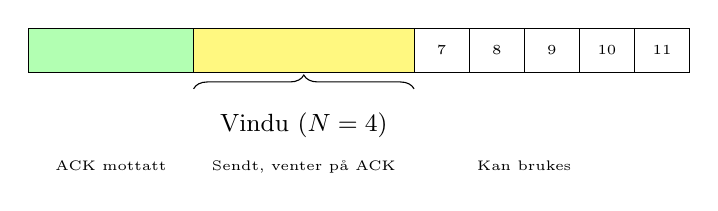
\begin{tikzpicture}[scale=0.7]
    \foreach \i in {0,...,11} {
        \draw (\i,0) rectangle (\i+1,0.8);
        \node at (\i+0.5,0.4) {\tiny \i};
    }
    \draw[fill=green!30] (0,0) rectangle (3,0.8);
    \draw[fill=yellow!50] (3,0) rectangle (7,0.8);

    \draw[decorate,decoration={brace,amplitude=5pt}] (3,-0.3) -- (7,-0.3) node[midway,below=5pt]{\small Vindu ($N=4$)};

    \node[below=1cm] at (1.5,0) {\tiny ACK mottatt};
    \node[below=1cm] at (5,0) {\tiny Sendt, venter p\aa\ ACK};
    \node[below=1cm] at (9,0) {\tiny Kan brukes};
\end{tikzpicture}
\end{center}

\subsection{Selective Repeat (SR)}

\begin{keybox}[Selective Repeat protokoll]
\textbf{Sender:}
\begin{itemize}[noitemsep]
    \item Vindu med opptil $N$ ubekreftede pakker
    \item \textbf{Individuell ACK:} Hver pakke har sin egen ACK
    \item Timer for \emph{hver} ubekreftet pakke
    \item Ved timeout: retransmitter kun den \emph{spesifikke} pakken som timet ut
\end{itemize}

\textbf{Mottaker:}
\begin{itemize}[noitemsep]
    \item Bekrefter \emph{hver} korrekt mottatt pakke individuelt
    \item \textbf{Bufferer} pakker mottatt ute av rekkef\o lge
    \item Leverer til applikasjonen n\aa r ``hullet'' fylles inn
\end{itemize}
\end{keybox}

\begin{warnbox}[SR-dilemmaet: Vindusst\o rrelse vs. sekvensnummerrom]
Vindusst\o rrelsen $N$ m\aa\ v\ae re \textbf{h\o yst halvparten av sekvensnummerrommet}:
\[
N \leq \frac{k}{2} \quad \text{der } k \text{ er antall mulige sekvensnumre}
\]
Ellers kan mottaker ikke skille mellom nye pakker og retransmisjoner!

\textbf{Eksempel:} Med sekvensnumre $\{0, 1, 2, 3\}$ (4 mulige) m\aa\ $N \leq 2$.
\end{warnbox}

\begin{center}
\begin{tabular}{lcc}
\toprule
\textbf{Egenskap} & \textbf{Go-Back-N} & \textbf{Selective Repeat} \\
\midrule
ACK-type & Kumulativ & Individuell \\
Mottaker-buffering & Nei & Ja \\
Ved timeout & Retransmitter alle & Retransmitter \'{e}n \\
Timer & \'{E}n (eldste) & Per pakke \\
Kompleksitet & Lavere & H\o yere \\
Effektivitet & Lavere (mange retransm.) & H\o yere \\
\bottomrule
\end{tabular}
\end{center}

%=============================================================================
\section{Tilkoblingsorientert transport: TCP (3.5)}
%=============================================================================

\subsection{TCP -- oversikt}

\begin{keybox}[TCP -- Egenskaper]
\begin{itemize}[noitemsep]
    \item \textbf{Punkt-til-punkt:} \'{E}n sender, \'{e}n mottaker
    \item \textbf{P\aa litelig, ordnet bytestr\o m:} Ingen meldingsgrenser
    \item \textbf{Full dupleks:} Data kan flyte begge veier samtidig (bi-directional data flow)
    \item \textbf{Kumulativ ACK}
    \item \textbf{Pipelining:} Vindusstyrte segmenter (congestion \& flow control setter vindu)
    \item \textbf{Tilkoblingsorientert:} H\aa ndtrykk (handshake) f\o r datautveksling
    \item \textbf{Flyt- og metningskontroll:} Sender overbelaster ikke mottaker eller nettverk
\end{itemize}
\end{keybox}

\subsection{TCP-segmentstruktur}

\begin{center}
\begin{tikzpicture}[scale=0.75]
    % Row 1 - Source/Dest port
    \draw[fill=lightblue] (0,6) rectangle (4,7);
    \draw[fill=lightblue] (4,6) rectangle (8,7);
    \node at (2,6.5) {\small Kilde-portnr (16 bit)};
    \node at (6,6.5) {\small Dest.-portnr (16 bit)};

    % Row 2 - Sequence number
    \draw[fill=lightblue] (0,5) rectangle (8,6);
    \node at (4,5.5) {\small Sekvensnummer (32 bit)};

    % Row 3 - ACK number
    \draw[fill=lightblue] (0,4) rectangle (8,5);
    \node at (4,4.5) {\small Bekreftelsesnummer / ACK-nummer (32 bit)};

    % Row 4 - Header length, flags, receive window
    \draw[fill=lightyellow] (0,3) rectangle (2,4);
    \draw[fill=lightyellow] (2,3) rectangle (4.5,4);
    \draw[fill=lightyellow] (4.5,3) rectangle (8,4);
    \node at (1,3.5) {\tiny Head len};
    \node at (3.25,3.5) {\tiny C E U A P R S F};
    \node at (6.25,3.5) {\small Receive window (16 bit)};

    % Row 5 - Checksum, Urgent pointer
    \draw[fill=lightblue] (0,2) rectangle (4,3);
    \draw[fill=lightblue] (4,2) rectangle (8,3);
    \node at (2,2.5) {\small Sjekksum (16 bit)};
    \node at (6,2.5) {\small Urgentpeker (16 bit)};

    % Row 6 - Options
    \draw[fill=lightyellow] (0,1) rectangle (8,2);
    \node at (4,1.5) {\small Opsjoner (variabel lengde)};

    % Row 7 - Data
    \draw[fill=lightgreen] (0,-0.5) rectangle (8,1);
    \node at (4,0.25) {\small Applikasjonsdata (variabel lengde)};

    % Brace for header
    \draw[decorate,decoration={brace,amplitude=5pt}] (-0.3,1) -- (-0.3,7) node[midway,left=5pt,align=center]{\small 20 byte\\[-2pt]\small header\\[-2pt]\small (min.)};

    % Width annotation
    \draw[decorate,decoration={brace,amplitude=5pt,mirror}] (0,7.2) -- (8,7.2) node[midway,above=5pt]{\small 32 bit};
\end{tikzpicture}
\end{center}

\begin{keybox}[Viktige felt i TCP-headeren]
\begin{itemize}[noitemsep]
    \item \textbf{Sekvensnummer:} Bytenummer til f\o rste byte i segmentets data
    \item \textbf{ACK-nummer:} Neste byte mottakeren forventer (kumulativ ACK)
    \item \textbf{Receive window (rwnd):} Antall byte mottaker er villig til \aa\ akseptere (flytkontroll)
    \item \textbf{Flagg:} SYN, FIN, ACK, RST, PSH, URG, CWR, ECE
    \item \textbf{Header-lengde:} Variabel pga. opsjoner (normalt 20 byte uten opsjoner)
\end{itemize}
\end{keybox}

\subsection{MSS og MTU}

\begin{formulabox}[MSS og MTU]
\begin{itemize}[noitemsep]
    \item \textbf{MTU (Maximum Transmission Unit):} St\o rste linklags-ramme (typisk \textbf{1500 byte} for Ethernet)
    \item \textbf{MSS (Maximum Segment Size):} Maks applikasjonsdata i segment
    \item $\text{MSS} = \text{MTU} - \text{IP-header} - \text{TCP-header} = 1500 - 20 - 20 = \textbf{1460 byte}$
    \item MSS refererer til applikasjonsdata, \emph{ikke} inkludert TCP-header
\end{itemize}
\end{formulabox}

\subsection{TCP sekvensnumre og ACK}

\begin{keybox}[Sekvensnumre og ACK i TCP]
\textbf{Sekvensnumre:}
\begin{itemize}[noitemsep]
    \item TCP nummererer \emph{byte} (ikke segmenter!)
    \item Sekvensnummeret er bytenummeret til f\o rste databyte i segmentet
    \item Eksempel: fil p\aa\ 500\,000 byte, MSS = 1000 byte $\Rightarrow$ segment 0 har seq=0, segment 1 har seq=1000, segment 2 har seq=2000, \ldots
\end{itemize}

\textbf{ACK-numre:}
\begin{itemize}[noitemsep]
    \item ACK-nummeret er sekvensnummeret til \textbf{neste byte mottakeren forventer}
    \item \textbf{Kumulativ ACK:} Bekrefter alle byte t.o.m. ACK-nummer $-$ 1
    \item Sp\o rsm\aa l: Hva gj\o r mottaker med pakker ute av rekkef\o lge? TCP-spec sier ingenting -- opp til implementasjon (i praksis: buffer dem)
\end{itemize}
\end{keybox}

\begin{exambox}[Eksempel: Telnet-sesjon]
Vert A sender `C' (1 byte) til Vert B, begge starter med seq=42 (A) og seq=79 (B):
\begin{enumerate}[noitemsep]
    \item A $\rightarrow$ B: Seq=42, ACK=79, data=`C'
    \item B $\rightarrow$ A: Seq=79, ACK=43, data=`C' (ekko)
    \item A $\rightarrow$ B: Seq=43, ACK=80
\end{enumerate}
\end{exambox}

\subsection{TCP Round-Trip Time og timeout}

\begin{formulabox}[RTT-estimering og timeout]
\textbf{SampleRTT:} M\aa lt tid fra segment sendt til ACK mottatt (kun for segmenter sendt \'{e}n gang).

\textbf{Estimert RTT (eksponensielt vektet glidende gjennomsnitt -- EWMA):}
\[
\text{EstimatedRTT} = (1 - \alpha) \cdot \text{EstimatedRTT} + \alpha \cdot \text{SampleRTT}
\]
Typisk: $\alpha = 0{,}125$ (dvs. $1/8$)

\textbf{Avviksm\aa l (Safety margin):}
\[
\text{DevRTT} = (1 - \beta) \cdot \text{DevRTT} + \beta \cdot |\text{SampleRTT} - \text{EstimatedRTT}|
\]
Typisk: $\beta = 0{,}25$ (dvs. $1/4$)

\textbf{Timeout-intervall:}
\[
\text{TimeoutInterval} = \text{EstimatedRTT} + 4 \cdot \text{DevRTT}
\]
\end{formulabox}

\begin{warnbox}[Viktig om SampleRTT]
SampleRTT m\aa les \textbf{ikke} for retransmitterte segmenter (Karn's algoritme) -- man kan ikke vite om ACK-en er for originalen eller retransmisjonen.
\end{warnbox}

\subsection{TCP p\aa litelig dataoverf\o ring}

\begin{keybox}[TCP sender -- forenklet]
TCP bruker \textbf{\'{e}n retransmissjonstimer} per tilkobling (ikke per segment).

\textbf{Hendelser hos sender:}
\begin{enumerate}[noitemsep]
    \item \textbf{Data fra applikasjon:} Lag segment med sekvensnummer, start timer hvis ikke allerede kj\o rende
    \item \textbf{Timeout:} Retransmitter segmentet med lavest sekvensnummer som ikke er bekreftet. Start timer p\aa\ nytt
    \item \textbf{ACK mottatt:} Hvis ACK bekrefter tidligere ubekreftede segmenter -- oppdater hva som er bekreftet. Start timer p\aa\ nytt hvis det fortsatt er ubekreftede segmenter
\end{enumerate}
\end{keybox}

\begin{keybox}[TCP fast retransmit]
Hvis sender mottar \textbf{3 duplikat-ACKer} (dvs.\ 4 ACKer for samme segment): retransmitter segmentet \emph{f\o r timeout} utl\o per.

Rasjonale: Duplikat-ACKer indikerer at et segment har g\aa tt tapt, men etterfølgende segmenter har kommet frem.
\end{keybox}

\subsection{TCP flytkontroll}

\begin{keybox}[Flytkontroll -- Flow Control]
\textbf{M\aa l:} Sender skal ikke oversvjemme mottakers buffer.

\textbf{Mekanisme:}
\begin{itemize}[noitemsep]
    \item Mottaker annonserer ledig bufferplass i TCP-headeren via \textbf{rwnd}-feltet (receive window)
    \item $\text{rwnd} = \text{RcvBuffer} - (\text{LastByteRcvd} - \text{LastByteRead})$
    \item Sender begrenser ubekreftede data: $\text{LastByteSent} - \text{LastByteAcked} \leq \text{rwnd}$
    \item Standard RcvBuffer = 4096 byte (kan \o kes via operativsystem)
\end{itemize}
\end{keybox}

\begin{warnbox}[Hva n\aa r rwnd = 0?]
N\aa r mottaker annonserer $\text{rwnd} = 0$, sender sender fortsatt sm\aa\ \textbf{probe-segmenter} (1 byte) for \aa\ f\aa\ oppdatert rwnd-verdi og unng\aa\ deadlock.
\end{warnbox}

\subsection{TCP tilkoblingsadministrasjon}

\subsubsection{Treveis h\aa ndtrykk (3-way handshake)}

\begin{keybox}[TCP tilkoblingsoppsett -- 3-veis h\aa ndtrykk]
\begin{enumerate}[noitemsep]
    \item \textbf{SYN:} Klient sender SYN-segment (SYN=1, velger tilfeldig sekvensnummer \texttt{client\_isn})
    \item \textbf{SYN-ACK:} Server svarer med SYNACK (SYN=1, ACK=1, velger \texttt{server\_isn}, acker \texttt{client\_isn+1})
    \item \textbf{ACK:} Klient sender ACK (ACK=1, acker \texttt{server\_isn+1}). Kan inneholde data!
\end{enumerate}
\end{keybox}

\begin{center}
\begin{tikzpicture}[>=Stealth, scale=0.9]
    \draw[thick] (0,0) -- (0,-5) node[above right, at start]{\textbf{Klient}};
    \draw[thick] (7,0) -- (7,-5) node[above left, at start]{\textbf{Server}};

    \draw[->, blue, thick] (0,-1) -- (7,-2) node[midway, above, sloped]{\small SYN, Seq=x};
    \draw[->, red, thick] (7,-2) -- (0,-3) node[midway, above, sloped]{\small SYN-ACK, Seq=y, ACK=x+1};
    \draw[->, blue, thick] (0,-3) -- (7,-4) node[midway, above, sloped]{\small ACK, Seq=x+1, ACK=y+1};

    \node[left] at (0,-1) {\tiny SYN\_SENT};
    \node[right] at (7,-2) {\tiny SYN\_RCVD};
    \node[left] at (0,-3) {\tiny ESTABLISHED};
    \node[right] at (7,-4) {\tiny ESTABLISHED};
\end{tikzpicture}
\end{center}

\begin{warnbox}[Hvorfor ikke toveis h\aa ndtrykk?]
Et toveis h\aa ndtrykk feiler fordi:
\begin{itemize}[noitemsep]
    \item Variable forsinkelser -- retransmitterte meldinger kan ankomme etter at tilkoblingen er lukket
    \item Meldinger kan komme i feil rekkef\o lge
    \item Kan ikke ``se'' den andre siden -- \textbf{halvåpne tilkoblinger} oppst\aa r
\end{itemize}
\end{warnbox}

\subsubsection{Tilkoblingslukking}

\begin{keybox}[TCP tilkoblingslukking -- 4-stegs prosess]
\begin{enumerate}[noitemsep]
    \item Klient sender \textbf{FIN}-segment
    \item Server svarer med \textbf{ACK} (halvlukket -- server kan fortsatt sende data)
    \item Server sender \textbf{FIN}-segment
    \item Klient svarer med \textbf{ACK}, g\aa r inn i \textbf{TIME\_WAIT} (venter typisk 2 $\times$ MSL)
\end{enumerate}
\end{keybox}

\begin{center}
\begin{tikzpicture}[>=Stealth, scale=0.9]
    \draw[thick] (0,0) -- (0,-7) node[above right, at start]{\textbf{Klient}};
    \draw[thick] (7,0) -- (7,-7) node[above left, at start]{\textbf{Server}};

    \draw[->, blue, thick] (0,-0.5) -- (7,-1.5) node[midway, above, sloped]{\small FIN};
    \draw[->, red, thick] (7,-1.5) -- (0,-2.5) node[midway, above, sloped]{\small ACK};
    \draw[->, red, thick] (7,-3.5) -- (0,-4.5) node[midway, above, sloped]{\small FIN};
    \draw[->, blue, thick] (0,-4.5) -- (7,-5.5) node[midway, above, sloped]{\small ACK};

    \node[left] at (0,-0.5) {\tiny FIN\_WAIT\_1};
    \node[left] at (0,-2.5) {\tiny FIN\_WAIT\_2};
    \node[left] at (0,-4.5) {\tiny TIME\_WAIT};
    \node[right] at (7,-1.5) {\tiny CLOSE\_WAIT};
    \node[right] at (7,-3.5) {\tiny LAST\_ACK};
    \node[right] at (7,-5.5) {\tiny CLOSED};

    \draw[dashed] (0,-4.5) -- (0,-6.5) node[left, midway]{\tiny Venter 2$\times$MSL};
    \node[left] at (0,-6.5) {\tiny CLOSED};
\end{tikzpicture}
\end{center}

\subsubsection{TCP-tilstander}

\begin{center}
\begin{tabular}{ll}
\toprule
\textbf{Tilstand} & \textbf{Beskrivelse} \\
\midrule
CLOSED & Ingen tilkobling \\
LISTEN & Server venter p\aa\ innkommende SYN \\
SYN\_SENT & Klient har sendt SYN, venter p\aa\ SYN-ACK \\
SYN\_RCVD & Server har mottatt SYN, sendt SYN-ACK \\
ESTABLISHED & Tilkobling etablert, data kan overf\o res \\
FIN\_WAIT\_1 & Har sendt FIN, venter p\aa\ ACK \\
FIN\_WAIT\_2 & FIN bekreftet, venter p\aa\ FIN fra andre side \\
CLOSE\_WAIT & Mottatt FIN, venter p\aa\ at applikasjonen lukker \\
LAST\_ACK & Sendt FIN, venter p\aa\ siste ACK \\
TIME\_WAIT & Venter 2$\times$MSL f\o r \aa\ sikre at siste ACK mottas \\
\bottomrule
\end{tabular}
\end{center}

%=============================================================================
\section{Prinsipper for metningskontroll (3.6)}
%=============================================================================

\subsection{Hva er metning (congestion)?}

\begin{keybox}[Metning -- Congestion]
\textbf{Metning} oppst\aa r n\aa r for mange kilder sender for mye data for fort, slik at \textbf{nettverket} ikke klarer \aa\ h\aa ndtere alt.

\textbf{Symptomer:}
\begin{itemize}[noitemsep]
    \item Lange k\o forsinkelser (k\o er i ruterbuffere)
    \item Pakketap (buffer-overflyt i rutere)
\end{itemize}

\textbf{Forskjell fra flytkontroll:}
\begin{itemize}[noitemsep]
    \item \textbf{Flytkontroll:} Hindrer sender i \aa\ oversvjemme \emph{mottaker}
    \item \textbf{Metningskontroll:} Hindrer sender i \aa\ oversvjemme \emph{nettverket}
\end{itemize}
\end{keybox}

\subsection{Kostnader ved metning}

\begin{warnbox}[Kostnader ved metning]
\begin{itemize}[noitemsep]
    \item K\o forsinkelser \o ker n\aa r ankomsthastighet n\ae rmer seg linkkapasitet
    \item Retransmisjoner pga.\ pakketap -- ``wasted'' arbeid
    \item Un\o dvendige retransmisjoner (premature timeout) -- senderen sender \emph{kopier} av pakker som allerede er levert
    \item N\aa r en pakke droppes langs en sti, g\aa r all oppadg\aa ende overf\o ringskapasitet brukt p\aa\ den pakken til spille
\end{itemize}
\end{warnbox}

\subsection{Tilnm\ae rminger til metningskontroll}

\begin{keybox}[To hovedtilnm\ae rminger]
\textbf{1. End-to-end metningskontroll:}
\begin{itemize}[noitemsep]
    \item Ingen eksplisitt tilbakemelding fra nettverket
    \item Metning utledes fra observert tap og forsinkelse
    \item TCP bruker denne tilnm\ae rmingen
\end{itemize}

\textbf{2. Nettverksassistert metningskontroll:}
\begin{itemize}[noitemsep]
    \item Rutere gir tilbakemelding til sender
    \item Kan v\ae re \emph{direkte} (eksplisitt rate) eller \emph{indirekte} (ECN-bit i header)
    \item ECN (Explicit Congestion Notification): 2 bit i IP-headeren
\end{itemize}
\end{keybox}

%=============================================================================
\section{TCP metningskontroll (3.7)}
%=============================================================================

\subsection{Oversikt: CWND og RWND}

\begin{keybox}[De to ``bremsene'' i TCP]
TCP-sender begrenser overf\o ringshastigheten med to vinduer:
\begin{itemize}[noitemsep]
    \item \textbf{cwnd (Congestion Window):} Bestemt av \emph{senderen} basert p\aa\ observert metning. \emph{Ikke} synlig i headeren (intern variabel)
    \item \textbf{rwnd (Receive Window):} Bestemt av \emph{mottakeren}, annonsert i TCP-headeren
\end{itemize}

\textbf{Den gylne regel:}
\[
\text{LastByteSent} - \text{LastByteAcked} \leq \min(\text{cwnd}, \text{rwnd})
\]

\textbf{TCP senderate:}
\[
\text{rate} \approx \frac{\text{cwnd}}{\text{RTT}} \text{ bytes/sek}
\]
\end{keybox}

\begin{formulabox}[B\aa ndbredde med og uten metningskontroll]
\textbf{Uten} metningskontroll (pre-Tahoe):
\[
BW_i = \frac{\text{TCP Window}}{\text{RTT}} = \frac{\text{RWND} \cdot \text{MSS}}{\text{RTT}}
\]

\textbf{Med} metningskontroll:
\[
BW_i = \frac{\text{TCP Window}}{\text{RTT}} = \frac{\min(\text{CWND}, \text{RWND}) \cdot \text{MSS}}{\text{RTT}}
\]
\end{formulabox}

\subsection{TCP Slow Start}

\begin{keybox}[Slow Start -- Eksponentiell vekst]
Ved \textbf{tilkoblingsstart}:
\begin{itemize}[noitemsep]
    \item $\text{cwnd} = 1$ MSS
    \item Initial rate = MSS/RTT
    \item For \textbf{hver mottatt ACK}: $\text{cwnd} = \text{cwnd} + \text{MSS}$
    \item Resulterer i \textbf{dobling} av cwnd per RTT (eksponentiell vekst)
\end{itemize}

\textbf{Eksempel} (MSS = 500 bytes, RTT = 200 ms):\\
Initial rate = 500/0{,}2 = 20 kbps, men dobles for hver RTT.
\end{keybox}

\begin{exambox}[Slow Start beregning]
Om cwnd = 4500 og MSS = 1500:\\
Det sendes 4500/1500 = 3 segmenter, og det kommer 3 ACK denne RTT:
\begin{itemize}[noitemsep]
    \item ACK 1: cwnd = 4500 + 1500 = 6000
    \item ACK 2: cwnd = 6000 + 1500 = 7500
    \item ACK 3: cwnd = 7500 + 1500 = 9000
\end{itemize}
Dvs.\ cwnd \textbf{doblet} fra 4500 til 9000 p\aa\ \'{e}n RTT!
\end{exambox}

\subsection{Congestion Avoidance -- AIMD}

\begin{keybox}[Congestion Avoidance -- Line\ae r vekst]
N\aa r cwnd $\geq$ ssthresh (slow start threshold):
\begin{itemize}[noitemsep]
    \item \textbf{Additive Increase:} For hver mottatt ACK:
    \[
    \text{cwnd} = \text{cwnd} + \text{MSS} \cdot \frac{\text{MSS}}{\text{cwnd}}
    \]
    Resulterer i \o kning p\aa\ \textbf{1 MSS per RTT} (line\ae r vekst)
    \item \textbf{Multiplicative Decrease:} Ved pakketap: halver cwnd
\end{itemize}
Gir ``sagtann''-m\o nster (\emph{saw tooth behavior}) -- prober stadig etter ledig b\aa ndbredde.
\end{keybox}

\begin{exambox}[Congestion Avoidance beregning]
Om cwnd = 3000 og MSS = 1500 (i Congestion Avoidance):
\begin{itemize}[noitemsep]
    \item cwnd0 = 3000 (start av RTT)
    \item Det sendes 3000/1500 = 2 segmenter $\Rightarrow$ 2 ACK
    \item ACK 1: cwnd = 3000 + 1500$\cdot$(1500/3000) = 3000 + 750 = 3750
    \item ACK 2: cwnd = 3750 + 1500$\cdot$(1500/3750) = 3750 + 600 = 4350
\end{itemize}
Dvs.\ cwnd \o kte med ca.\ \textbf{1 MSS} til neste RTT (line\ae r vekst). (Eksakt 1 MSS ved start av neste RTT-periode.)
\end{exambox}

\subsection{Tapshendelser og ssthresh}

\begin{keybox}[Reaksjon p\aa\ tap -- ssthresh]
Variabelen \textbf{ssthresh} (slow start threshold) avgj\o r n\aa r man g\aa r fra Slow Start til Congestion Avoidance.

\textbf{Ved tapshendelse:}
\begin{itemize}[noitemsep]
    \item $\text{ssthresh} = \text{cwnd} / 2$
\end{itemize}

\textbf{To typer tap -- ulik respons:}

\textbf{1. Timeout:}
\begin{itemize}[noitemsep]
    \item ssthresh = cwnd/2
    \item cwnd = 1 MSS
    \item G\aa\ tilbake til \textbf{Slow Start}
\end{itemize}

\textbf{2. Trippel duplikat-ACK (3 dup ACK):}
\begin{itemize}[noitemsep]
    \item ssthresh = cwnd/2
    \item cwnd = ssthresh + 3 MSS
    \item G\aa\ inn i \textbf{Fast Recovery}
\end{itemize}
\end{keybox}

\subsection{De tre mekanismene i TCP metningskontroll}

\begin{center}
\begin{tikzpicture}[>=Stealth, scale=0.85,
    state/.style={draw, rounded corners, fill=lightblue, minimum width=3cm, minimum height=1.2cm, align=center, font=\small\bfseries}]

    \node[state] (ss) at (0,0) {Slow\\Start};
    \node[state] (ca) at (6,0) {Congestion\\Avoidance};
    \node[state] (fr) at (3,-4) {Fast\\Recovery};

    % SS -> CA
    \draw[->, thick] (ss) -- (ca) node[midway, above, font=\scriptsize]{cwnd $\geq$ ssthresh};

    % SS -> SS (timeout)
    \draw[->, thick] (ss) to[loop left] node[left, font=\scriptsize, align=right]{timeout:\\ssthresh=cwnd/2\\cwnd=1 MSS} (ss);

    % CA -> SS (timeout)
    \draw[->, thick] (ca) to[bend right=30] node[above, font=\scriptsize, align=center]{timeout:\\ssthresh=cwnd/2\\cwnd=1 MSS} (ss);

    % SS -> FR (3 dup ACK)
    \draw[->, thick] (ss) to[bend right=20] node[left, font=\scriptsize, align=right]{3 dup ACK:\\ssthresh=cwnd/2\\cwnd=ssthresh+3} (fr);

    % CA -> FR (3 dup ACK)
    \draw[->, thick] (ca) -- (fr) node[right, font=\scriptsize, align=left]{3 dup ACK:\\ssthresh=cwnd/2\\cwnd=ssthresh+3};

    % FR -> CA (new ACK)
    \draw[->, thick] (fr) to[bend right=20] node[right, font=\scriptsize, align=left]{New ACK:\\cwnd=ssthresh} (ca);

    % FR -> SS (timeout)
    \draw[->, thick] (fr) to[bend right=20] node[below, font=\scriptsize, align=center]{timeout:\\ssthresh=cwnd/2, cwnd=1} (ss);
\end{tikzpicture}
\end{center}

\subsection{TCP Tahoe vs. TCP Reno}

\begin{keybox}[TCP Tahoe vs. TCP Reno]
\textbf{TCP Tahoe (1988):}
\begin{itemize}[noitemsep]
    \item Ved \emph{alle} tapshendelser (b\aa de timeout og 3 dup ACK): cwnd = 1 MSS, g\aa\ til Slow Start
\end{itemize}

\textbf{TCP Reno (1997, RFC 2001/2581):}
\begin{itemize}[noitemsep]
    \item Ved \textbf{timeout}: cwnd = 1 MSS, g\aa\ til Slow Start (som Tahoe)
    \item Ved \textbf{3 dup ACK}: cwnd = ssthresh + 3, g\aa\ til Fast Recovery (mildere reaksjon)
    \item Fast Recovery gir bedre ytelse -- pakketap via dup-ACK betyr at nettverket fortsatt leverer noen pakker
\end{itemize}
\end{keybox}

\subsection{TCP CUBIC}

\begin{keybox}[TCP CUBIC -- Moderne metningskontroll]
TCP CUBIC er \textbf{standard i Linux} og den mest brukte TCP-varianten for webservere.

\textbf{Motivasjon:} Klassisk AIMD (line\ae r \o kning) er for treg n\aa r b\aa ndbredden er h\o y.

\textbf{Iid\'{e}:}
\begin{itemize}[noitemsep]
    \item $W_{\max}$ = senderate da metning sist ble oppdaget
    \item Etter halvering av cwnd: \o k raskt tilbake mot $W_{\max}$, men sakk ned n\ae r $W_{\max}$
    \item $K$ = tidspunkt da vinduet n\aa r $W_{\max}$ (konfigurerbar)
    \item \O kning av $W$ som funksjon av \textbf{kuben} av avstanden mellom n\aa v\ae rende tid og $K$
    \item St\o rre \o kninger n\aa r langt fra $K$, mindre \o kninger n\ae r $K$ (forsiktig)
\end{itemize}

\textbf{Fordeler:}
\begin{itemize}[noitemsep]
    \item Uavhengig av RTT (bruker veggklokketid)
    \item Rettferdig p\aa\ tvers av ulike RTT-er
    \item H\o yere gjennomstr\o mning enn klassisk TCP p\aa\ h\o yhastighetslenker
\end{itemize}
\end{keybox}

\subsection{TCP Fairness -- Rettferdighet}

\begin{keybox}[TCP Fairness]
\textbf{M\aa l:} Hvis $K$ TCP-sesjoner deler en flaskehalslenke med kapasitet $R$, b\o r hver f\aa\ gjennomsnittlig rate $R/K$.

\textbf{Hvorfor AIMD gir rettferdighet:}
\begin{itemize}[noitemsep]
    \item Additive Increase: begge sesjoner \o ker med stigning 1 (parallelt med likedelingslinjen)
    \item Multiplicative Decrease: begge halverer (beveger seg mot likedelingslinjen)
    \item Over tid konvergerer sesjonene mot lik andel av b\aa ndbredden
\end{itemize}

\textbf{NB:} Dette er et veldig teoretisk resultat -- i praksis p\aa virker RTT, antall tilkoblinger per applikasjon, og UDP-trafikk (som ikke har metningskontroll) rettferdigheten.
\end{keybox}

\subsection{Bottleneck-lenken}

\begin{warnbox}[Bottleneck-lenke og TCP-oppf\o rsel]
TCP (\aa de klassisk og CUBIC) \o ker senderaten til pakketap oppst\aa r ved en ruters utgang -- \textbf{bottleneck-lenken}.

\textbf{Viktige innsikter:}
\begin{itemize}[noitemsep]
    \item \O kt TCP-senderate \textbf{vil ikke} \o ke ende-til-ende-gjennomstr\o mning n\aa r bottleneck er mettet
    \item \O kt senderate \textbf{vil} \o ke m\aa lt RTT (pga. k\o er)
    \item M\aa l: ``Hold ende-til-ende-r\o ret akkurat fullt, men ikke fullere''
\end{itemize}
\end{warnbox}

%=============================================================================
\section{Evolusjon av transportlags-funksjonalitet (3.8)}
%=============================================================================

\subsection{Utfordringer med TCP}

\begin{keybox}[Ulike scenarier -- ulike utfordringer]
\begin{center}
\begin{tabular}{ll}
\toprule
\textbf{Scenario} & \textbf{Utfordring} \\
\midrule
Lange, fete r\o r (store dataoverf\o ringer) & Mange pakker ``in flight''; tap stopper pipeline \\
Tr\aa dl\o se nettverk & Tap pga.\ st\o y tolkes som metning \\
Lange forsinkelser & Ekstremt lang RTT \\
Datasenternettverk & Latens-sensitiv \\
Bakgrunnstrafikk & Lav-prioritets TCP-flyter \\
\bottomrule
\end{tabular}
\end{center}
\end{keybox}

\subsection{QUIC -- Quick UDP Internet Connections}

\begin{keybox}[QUIC og HTTP/3]
\textbf{QUIC} er en applikasjonslags-protokoll bygget \textbf{over UDP} som gir:
\begin{itemize}[noitemsep]
    \item P\aa litelig dataoverf\o ring
    \item Metningskontroll
    \item Autentisering og kryptering
    \item Tilkoblingsoppsett p\aa\ \textbf{1 RTT} (vs. TCP+TLS = 2 serielleh\aa ndtrykk)
\end{itemize}

\textbf{HTTP/3 = HTTP/2 (slanket) over QUIC over UDP}

\textbf{Fordeler over TCP:}
\begin{itemize}[noitemsep]
    \item Flere applikasjonsniv\aa\ ``str\o mmer'' multiplekset over \'{e}n QUIC-tilkobling
    \item Str\o mmene er \textbf{uavhengige} -- unng\aa r TCPs head-of-line blocking
    \item Separat p\aa litelig overf\o ring og sikkerhet per str\o m
    \item Felles metningskontroll p\aa\ tvers av str\o mmer
\end{itemize}
\end{keybox}

\begin{center}
\begin{tikzpicture}[scale=0.8]
    % HTTP/2 over TCP stack
    \node at (2, 4.5) {\textbf{HTTP/2 over TCP}};
    \draw[fill=lightblue] (0,3) rectangle (4,4);
    \node at (2,3.5) {\small HTTP/2};
    \draw[fill=lightyellow] (0,2) rectangle (4,3);
    \node at (2,2.5) {\small TLS};
    \draw[fill=lightgreen] (0,1) rectangle (4,2);
    \node at (2,1.5) {\small TCP};
    \draw[fill=lightred!50] (0,0) rectangle (4,1);
    \node at (2,0.5) {\small IP};

    % HTTP/3 over QUIC stack
    \node at (7, 4.5) {\textbf{HTTP/3 over QUIC}};
    \draw[fill=lightblue] (5,3) rectangle (9,4);
    \node at (7,3.5) {\small HTTP/2 (slanket)};
    \draw[fill=lightyellow] (5,2) rectangle (9,3);
    \node at (7,2.5) {\small QUIC};
    \draw[fill=lightgreen] (5,1) rectangle (9,2);
    \node at (7,1.5) {\small UDP};
    \draw[fill=lightred!50] (5,0) rectangle (9,1);
    \node at (7,0.5) {\small IP};

    % Labels
    \node[right] at (9.5, 3.5) {\scriptsize Applikasjon};
    \node[right] at (9.5, 1.5) {\scriptsize Transport};
    \node[right] at (9.5, 0.5) {\scriptsize Nettverk};
\end{tikzpicture}
\end{center}

\subsection{TCPs historiske utvikling}

\begin{center}
\begin{tabular}{lll}
\toprule
\textbf{\AA r} & \textbf{Milepæl} & \textbf{Kommentar} \\
\midrule
1980--81 & RFC 761 / RFC 793 & Opprinnelig TCP (kun Connection + Transfer) \\
1988 & TCP Tahoe (BSD) & Jacobson: Slow Start + Congestion Avoidance \\
1997 & TCP Reno (RFC 2001/2581) & Fast Retransmit + Fast Recovery \\
2005 & BIC TCP & Binm\ae r s\o k etter optimal vindusstm\o rrelse \\
2018 & TCP CUBIC & Kubisk funksjon, standard i Linux \\
\bottomrule
\end{tabular}
\end{center}

%=============================================================================
\section{Oppsummering}
%=============================================================================

\begin{keybox}[Kapittel 3 -- Hovedpunkter]
\begin{itemize}[noitemsep]
    \item \textbf{Transportlaget} gir logisk kommunikasjon mellom \emph{prosesser} (ikke verter)
    \item \textbf{Multipleksing/demultipleksing:} Portnumre dirigerer til riktig sokkel (UDP: 2-tuppel, TCP: 4-tuppel)
    \item \textbf{UDP:} Enkel, tilkoblingsl\o s, ``best effort'' -- bare mux/demux + sjekksum
    \item \textbf{P\aa litelig dataoverf\o ring:} Sjekksum, sekvensnumre, ACK, timer, retransmisjon
    \item \textbf{Pipelining:} GBN (kumulativ ACK, retransmitter alle) vs. SR (individuell ACK, buffer ute-av-rekkef\o lge)
    \item \textbf{TCP:} P\aa litelig, ordnet bytestr\o m med flytkontroll, metningskontroll og tilkoblingsadministrasjon
    \item \textbf{TCP metningskontroll:} Slow Start (eksponentiell), Congestion Avoidance (AIMD), Fast Recovery
    \item \textbf{TCP CUBIC:} Kubisk vindusm\o kning, standard i Linux, RTT-uavhengig
    \item \textbf{QUIC/HTTP/3:} Moderne alternativ over UDP med 1-RTT tilkobling og uavhengige str\o mmer
\end{itemize}
\end{keybox}

%=============================================================================
\section*{Formelsammendrag}
%=============================================================================

\begin{formulabox}[Alle viktige formler -- Kapittel 3]

\textbf{UDP sjekksum:} 1-er-komplement av summen av alle 16-biters ord.

\textbf{Stopp-og-vent utnyttelse:}
\[
U_{\text{sender}} = \frac{L/R}{RTT + L/R}
\]

\textbf{Pipelining utnyttelse ($n$ pakker):}
\[
U_{\text{sender}} = \frac{n \cdot L/R}{RTT + L/R}
\]

\textbf{MSS:}
\[
\text{MSS} = \text{MTU} - \text{IP-header} - \text{TCP-header} = 1500 - 20 - 20 = 1460 \text{ byte}
\]

\textbf{RTT-estimering:}
\begin{align*}
\text{EstimatedRTT} &= (1 - \alpha) \cdot \text{EstimatedRTT} + \alpha \cdot \text{SampleRTT} & (\alpha = 0{,}125) \\
\text{DevRTT} &= (1 - \beta) \cdot \text{DevRTT} + \beta \cdot |\text{SampleRTT} - \text{EstimatedRTT}| & (\beta = 0{,}25)
\end{align*}

\textbf{Timeout:}
\[
\text{TimeoutInterval} = \text{EstimatedRTT} + 4 \cdot \text{DevRTT}
\]

\textbf{TCP flytkontroll:}
\[
\text{rwnd} = \text{RcvBuffer} - (\text{LastByteRcvd} - \text{LastByteRead})
\]

\textbf{TCP sendebegrensning:}
\[
\text{LastByteSent} - \text{LastByteAcked} \leq \min(\text{cwnd}, \text{rwnd})
\]

\textbf{TCP senderate:}
\[
\text{rate} \approx \frac{\min(\text{cwnd}, \text{rwnd})}{\text{RTT}} \text{ bytes/sek}
\]

\textbf{Slow Start (per ACK):} cwnd = cwnd + MSS \quad (dobling per RTT)

\textbf{Congestion Avoidance (per ACK):} cwnd = cwnd + MSS $\cdot$ (MSS/cwnd) \quad (+1 MSS per RTT)

\textbf{Ved timeout:} ssthresh = cwnd/2, \quad cwnd = 1 MSS

\textbf{Ved 3 dup ACK:} ssthresh = cwnd/2, \quad cwnd = ssthresh + 3 MSS

\textbf{TCP fairness:} $K$ sesjoner, kapasitet $R$ $\Rightarrow$ hver f\aa r $R/K$

\textbf{SR vindusst\o rrelse:} $N \leq k/2$ der $k$ = antall sekvensnumre

\end{formulabox}
